\documentclass[border=6pt]{standalone}
\usepackage{tikz}
\usetikzlibrary{arrows.meta,positioning,fit,calc}
\definecolor{fg}{HTML}{3B3220}
\definecolor{fgbody}{HTML}{544736}
\definecolor{stroke}{HTML}{7A5A10}
\definecolor{surf}{HTML}{FAF6EE}
\definecolor{surfemph}{HTML}{F2E9D4}
\definecolor{surfact}{HTML}{F6E7E0}
\definecolor{bdim}{HTML}{CFC6B2}
\definecolor{bemph}{HTML}{7A5A10}
\definecolor{bact}{HTML}{8F1D1D}
\begin{document}
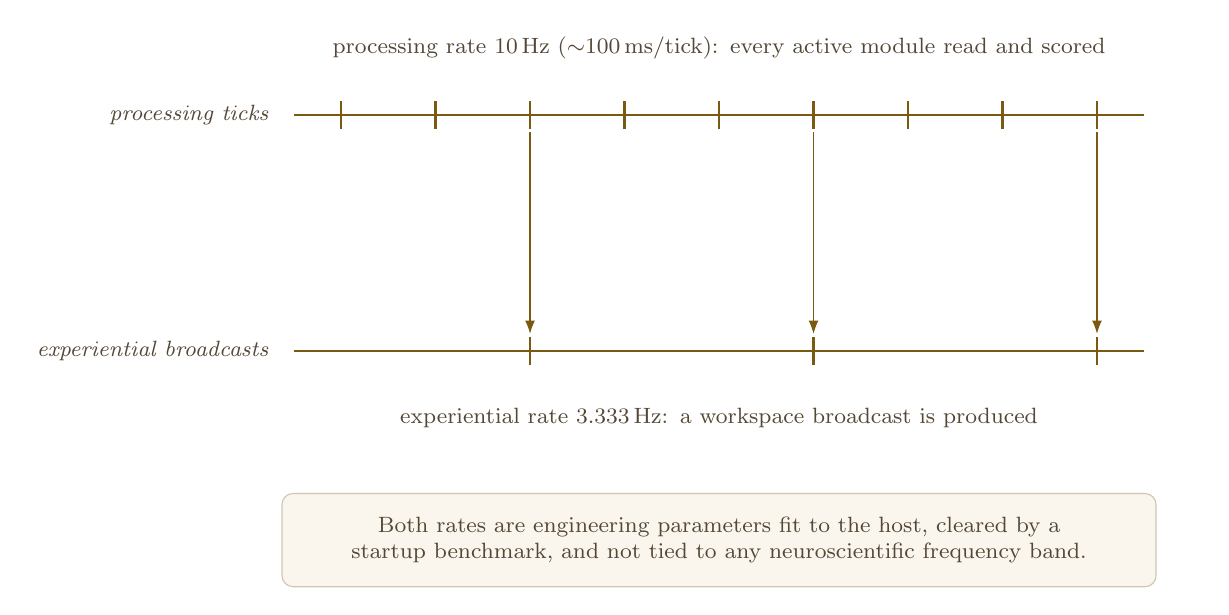
\begin{tikzpicture}[
  font=\small,>=Latex,
  every node/.append style={text=fgbody},
  tickmark/.style={draw=stroke, thick},
]
\def\upy{3.0}
\def\loy{0.0}
% --- upper track: processing ticks (10 Hz) ---
\draw[thick, draw=stroke] (-0.6,\upy) -- (10.2,\upy);
\foreach \i in {0,...,8} {
  \pgfmathsetmacro{\x}{\i*1.2}
  \draw[tickmark] (\x,\upy-0.18) -- (\x,\upy+0.18);
}
\node[align=center, font=\footnotesize, text width=120mm] at (4.8,\upy+0.85)
  {processing rate 10\,Hz ($\sim$100\,ms/tick): every active module read and scored};
% --- lower track: experiential broadcasts (3.333 Hz) ---
\draw[thick, draw=stroke] (-0.6,\loy) -- (10.2,\loy);
\foreach \x in {2.4,6.0,9.6} {
  \draw[tickmark] (\x,\loy-0.18) -- (\x,\loy+0.18);
}
\node[align=center, font=\footnotesize, text width=95mm] at (4.8,\loy-0.85)
  {experiential rate 3.333\,Hz: a workspace broadcast is produced};
% --- every third processing tick feeds a broadcast tick ---
\foreach \x in {2.4,6.0,9.6} {
  \draw[->, thin, draw=stroke] (\x,\upy-0.22) -- (\x,\loy+0.22);
}
% track labels
\node[font=\footnotesize\itshape, anchor=east] at (-0.8,\upy) {processing ticks};
\node[font=\footnotesize\itshape, anchor=east] at (-0.8,\loy) {experiential broadcasts};
% --- caption ---
\node[draw=bdim, rounded corners, fill=surf, align=center, font=\footnotesize, text width=105mm, inner sep=3mm] at (4.8,-2.4)
  {Both rates are engineering parameters fit to the host, cleared by a startup benchmark, and not tied to any neuroscientific frequency band.};
\end{tikzpicture}
\end{document}
